\Chapter{DLV és vizuális reprezentációja}

A modellen elvégzendő elemzések miatt szükséges lehet egy grafikus vizualizáció. A vizualizáció egyszerű, és érthető kell, hogy legyen. Vizualizálni sokféleképp lehet, jelen esetben a Python alá is elérhető GraphViz-re esett a választás. A GraphViz (Graph Visualization, a következőkben GV) egy gráf rajzoló program ami egy képfájlt állít elő a megadott paraméterből. A paraméter lehet szövegfájl, vagy valamilyen adatstruktúra. A GV egy saját leírónyelvvel is rendelkezik, de az "általános" gráfleírónyelvet (DOT) is használni tudja. Ez azért fontos, mert így lehet egy modul által feldolgozott adattömegből gráfot előállítani és azt vizualizálni.

Adott például egy DLV nevű nyelv. A neve az angol "DdataLog with disjunction (V)" kifejezésből származik. A DLV-t rendszerek alkatrészeként is jelen van. Ilyen például a nevéből alkotott DLV rendszer. A DLV rendszer [http://www.dlvsystem.com]  célja egy hatékony tudásreprezentációs modell, amely diszjunktív logikai alapokon, deklaratív megközelítéssel  biztosít  információ kezelést. A DLV rendszert, melyet a 1990-es évek közepén kezdtek el kidolgozni,  többek között az alábbi speciális funkciókkal rendelkezik: [Eiter, Thomas, et al. "Declarative problem-solving using the DLV system." Logic-based artificial intelligence. Springer, Boston, MA, 2000. 79-103.] 
\begin{itemize}
\item kirejesztett  disjunctive logic modul
\item a  strong negation művelet támogatása
\item kiterjesztett API felület 
\end{itemize}
A kibővített funkcionalitás viszont azt is eredményezte, hogy a logikai operátorok megvalósítása nem kellően hatékony a nagyobb méretű gyakorlati feladatok számára. A következtető motor hatékonyságának javítása folyamatosan a fejlesztések középpontjában áll, a DLV jelenlegi verziói már alkalmasak a közepes méretű feladatok megoldására.

A DLV a DL azaz Datalog nyelv kiterjesztése. A Datalog pedig a PROLOG nyelv egy részhalmazának tekinthető. A nyelv tartalmaz tényeket (facts), szabályokat (rules) és megkötéseket (constraint). Szabály felírható $$a_1 \wedge \ldots \wedge a_n \leftarrow b_1\vee \ldots \vee b_m \quad 1\leq n, 0\leq m$$ alakban. 
Vegyünk egy  példát! Adott egy monitor pixel. A pixel (P1,P2,P3,\ldots) lehet sokféle színű. De jelen esetben vegyük a komponenseket. A pixel fehér ha mindhárom komponense világit, vörös, ha csak a vörös, kék, ha csak a kék, és így tovább.  
Ez DATALOG-ban:
\begin{cpp}
blue(P1).
blue(P2).
blue(P3)
red(P2).
red(P3).
green(P3).

purple(X) :- blue(X), red(X), \+ green(X).
\end{cpp}
Tehát a pixel csak akkor lila ha csak a vörös és kék komponense világít (a példában feltesszük, hogy a komponensek intenzitása nem állítható.)Azért szükséges így megadni, mert egyébként a fehér pixel is lehetne lila. A $"\setminus+"$ operátor helyett szokás még a $"-"$ operátor használata is.
A diszjunkciót felhasználva DLV-ben az előbbi példa:
\begin{cpp}
blue(X) <- X=P1.
blue(X) <- X=P2.
blue(X) <- X=P3.
X=P1 v P2 v P3 <-blue(X).
\end{cpp}
Itt az első sor azt fejezi ki ha az objektumom a \textsl{P1}, akkor az objektum kék komponense be van kapcsolva. (2. és 3. sor analóg módon) Az utolsó sor pedig a modell alkotáshoz szükséges. Ugyanis ez azt fejezi ki, hogy ha egy objektum kék komponense világít, akkor az az objektum csak \textit{P1, P2} vagy \textit{P3} lehet. Ez azért szükséges, mert így elvetjük egy későbbi \textsl{P4} pixel "kékségét".
Folytatva a példát:
\begin{cpp}
red(X) <- X=P2.
red(X) <- X=P3.
X=P2 v P3 <- red(X).
\end{cpp}
A DLV hez tartozó adatbázis tartalmazza:
\begin{itemize}
\item tényeket leíró literálok
\item következtetési szabályok
\item integritási szabályok
\end{itemize}
Az integritási szabályok a következtetési szabályokhoz hasonló formátumúak, de üres a kötetkezmény része, például:
\begin{cpp}
<- blue(X) & red(X).
\end{cpp}
A DLV rendszer segítségével olyan  logikai  feladatok is megoldhatóak, mint a háromszín probléma,, vagyis adott térképet be tudunk-e színezni három szín segítségével, úgy.hogy a szomszédos területeket nem lehet azonos színnel jelölni. A megoldást természetesen egy adott problémára vonatkozóan oldható meg a DLV segítségével.\\
A szinezési probléma DLV  megfogalmazása $[forrás: http://www.dlvsystem.com/html/The_DLV_Tutorial.html]$
\begin{cpp}
node(minnesota).
node(wisconsin).
node(illinois).
node(iowa).
node(indiana).
node(michigan).
node(ohio).

arc(minnesota, wisconsin).
arc(illinois, iowa).
arc(illinois, michigan).
arc(illinois, wisconsin).
arc(illinois, indiana).
arc(indiana, ohio).
arc(michigan, indiana).
arc(michigan, ohio).
arc(michigan, wisconsin).
arc(minnesota, iowa).
arc(wisconsin, iowa).
arc(minnesota, michigan).

 % guess coloring
col(Country, red) v col(Country, green) v col(Country, blue) >:<
 :- node(Country).

% check coloring
:- arc(Country1, Country2), col(Country1, CommonColor), >:<
col(Country2, CommonColor). 
\end{cpp}
>:<\textit{ szerkesztési sortörés, a kódban nincs jelen}
A megoldás során keletkező modell:
\begin{cpp}
{col(minnesota,green), col(wisconsin,red), col(illinois,green),
 col(iowa,blue), col(indiana,red), col(michigan,blue), col(ohio,green)}
\end{cpp}
A DLV gyakorlati szerepét erősíti, hogy adatbázis  API  felülettel is rendelkezik, azaz a tények, interpretáció leírása hagyományos adatbázisokból is átvehetőek.  A beolvasó parancsban meg kell adni az adatsort meghatározó SQL parancsot és az itteni fogadó változókat:
\begin{cpp}
#import(dbAirports, "airportUser", "airportPasswd", >:< 
"SELECT * FROM flight_rel", flight, type : U_INT, Q_CONST,>:<
 Q_CONST, Q_CONST).
#import(dbCommercial, "commUser", "commPasswd", >:< 
"SELECT * FROM codeshare_rel", codeshare, type : Q_CONST, Q_CONST, U_INT).
#export(dbTravelAgency, "agencyName", "agencyPasswd", destinations, >:<
composedCompanyRoutes).

\end{cpp}
Mivel a  funkcionalitása alapján a  DLV rendszer egy fontos eszköznek tekinthető a deduktív rendszerek területén, vizsgálatainkhoz is ezt a rendszert választottuk ki.  
A DLV rendszer fejlesztése ma is aktívan vizsgált kutatási terület, melyet jól mutatnak az utóbbi években megjelent hozzá kapcsolódó tudományos munkák, melyek közül itt csak néhányat említünk meg:
\begin{itemize}
\item	Calimeri, Francesco, et al. "How Modern Deductive Database Systems Can Enhance Data Integration." SEBD. 2018.
\item Calimeri, Francesco, et al. "I-DLV: the new intelligent grounder of DLV." Intelligenza Artificiale 11.1 (2017): 5-20.
\item Cao, Son Thanh, and Linh Anh Nguyen. "Incorporating Stratified Negation into Query-Subquery Nets for Evaluating Queries to Stratified Deductive Databases." Computing and Informatics 38.1 (2019): 19-56.
\item Adrian, Weronika T., et al. "The ASP system DLV: advancements and applications." KI-Künstliche Intelligenz 32.2-3 (2018): 177-179.
\end{itemize}
A konverzió

A konverzió során a tényeket nem vesszük figyelembe, csak a szabályokat. Kihasználva, hogy a GraphViz (és sok más) megjelenítő képes DOT gráfok megjelenítésére, így a fő cél a DOT-ra történő konverzió. Egy egyszerű szabály két csomóponttal írható le. Az egyszerűbb követhetőség kedvéért, a tényeket fel lehet venni, így egy nyomtérképet készítve rendelkezésre álló tények segítségével. Ha így teszünk, akkor egy állítás konverziója  a következőképp történik:
\begin{table}[h!]
\centering
\begin{tabular}{|c|c|c|}
\hline
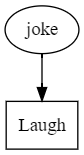
\includegraphics[scale=1]{images/joke1.png} & \textit{Ha viccet mondanak nevetünk.} &\texttt{Laugh(X) :- joke(X)} \\
\hline
\end{tabular}
\end{table}

\newpage
A következő lépés lekezelni az összetett szabályokat. Az összetett szabály állhat több előzményből és/vagy több következményből. Például, ha az illetőnk viccet hall, vagy vidám, akkor nevet. Ennek a megfordítása pedig, ha nevettünk, akkor viccet hallottunk, vagy vidámak voltunk. 
\begin{table}[h!]
\centering
\begin{tabular}{|c|c|c|}
\hline
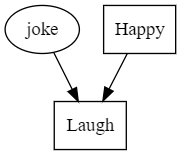
\includegraphics[scale=0.75]{images/joke2.png} & \textit{Ha viccet mondanak,  vagy boldogok vagyunk, akkor nevetünk} & \texttt{Laugh(X) :- joke(X) V Happy(X)}\\
\hline
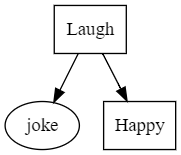
\includegraphics[scale=0.75]{images/joke3.png} & \textit{Ha nevettünk, akkor viccet mondtak, vagy jó kedvünk volt.}& \texttt{joke(X) V Happy(X) :- Laugh(X) }\\
\hline
\end{tabular}
\end{table}
A probléma akkor merül fel ha a szabály feje konjunkciót tartalmaz. Ekkor a képe ugyanis úgy nézne ki mint diszjunkció esetén, hiszen több feltétel egyidejűleg szükséges. Ezért szükséges egy ún. kötőelem bevezetése. Ezt úgy kell értelmezni, hogy a kötőelembe befutó éleknek egyidejűleg kell teljesülniük. 
\begin{center}
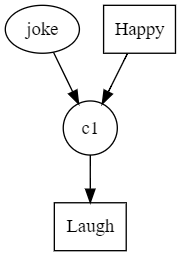
\includegraphics[scale=0.75]{images/joke4} 
\end{center}
Analóg módon a szabály másik részén található konjunkció is reprezentálható kötőelemmel. 